\newpage
\section{Evaluation} \label{sec:Evaluation}

Dieses Kapitel prüft das Artefakt aus \autoref{sec:Entwurf} gegen den Kriterienkatalog aus
\autoref{sec:kriterienkatalog}. U4 erhebt die Messgrößen S1 bis S4 und M5, U3 prüft M1 bis M4 über den
Prüffallkatalog und die Architekturprüfung. Grundlage sind Messläufe vom 6.\ bis zum 28.\ Oktober 2026. Den
Vergleich mit dem Ausgangszustand tragen allein die Läufe auf hyper-int-otc, die frühen Läufe dienten der Wahl der
Entwurfsparameter. Sie haben sechs Fehler in der Zustellung aufgedeckt, die \autoref{sec:zuverlaessigkeit} festhält.
Einzelne Detailtabellen stehen im \ref{sec:messdaten}.

\subsection{Messaufbau und Vorgehen}
\label{sec:messaufbau}

Gemessen wird auf dem Kubernetes-Cluster hyper-int-otc der Integrationsstufe (\autoref{tab:cluster}). Dort läuft
neben dem Prototyp der Ausgangszustand aus \autoref{sec:systemkontext}, je Mandant ein Knative-Service mit einem
Node.js-Runner, sodass beide Modelle auf demselben Cluster verglichen werden. Die Last stammt aus dem
Produktivbetrieb der AWS-nativen Variante und ist nur Quelle des Lastprofils.

\begin{table}[H]
  \caption{Der Cluster der Messungen}
  \label{tab:cluster}
  \small
  \begin{tabularx}{\textwidth}{@{}l >{\RaggedRight\arraybackslash}X@{}}
    \hline
    Knoten & 9 $\times$ s9.xlarge.4, zuletzt 8 \\
    Allokierbar & rund 71 Kerne, 243\,GiB \\
    NATS & 5 $\times$ NATS 2.14.0 \\
    Gemessen & Prototyp und Ausgangszustand \\
    gVisor & ja, Runtime-Klasse der Worker-Pods \\
    \hline
  \end{tabularx}
\end{table}

Der Prototyp lief in der Konfiguration aus \autoref{tab:parameter}, mit einer Pool-Zielgröße von vierzig und einer
Skalierungsschwelle von drei Vierteln, beide aus den ersten Läufen. Alle Läufe nutzen das Webhook-Profil mit
synchroner Antwort. Das Agentenprofil hat keinen Vergleichswert, weil es im Ausgangszustand nicht existiert.
\autoref{sec:kaltstart} nennt einen Richtwert. Die Prüffälle aus \autoref{sec:pruefung-isolation} laufen in beiden
Profilen.

Die Messungen stammen aus mehreren Ständen des Prototyps. Die vom 28.\ Oktober, also S1 mit Pool 40, der Overhead im
Lastprofil, M5 und die Prüffälle T7 und T9, laufen mit der Trennung in Transport und Sandbox aus
\autoref{sec:bausteine}, mit dem Egress-Proxy aus \autoref{sec:faehigkeitsmodell} in enforce für beide Profile, mit bis
zu vier Zustellungen (\autoref{sec:zuteilung}) und ohne Auth Callout, der auf der Plattform noch nicht eingerichtet ist.
Der Speicher je Pod stammt vom 26.\ Oktober, ohne Proxy, alle übrigen Messungen aus dem Stand davor. Die Abschnitte
nennen das Datum. Auf dem Stand seit dem 27.\ Oktober sind S3, S4, M3, T1 bis T6, T8 und SandboxEval nicht gemessen.
\autoref{tab:stand} im Anhang ordnet die Belege den Ständen zu.

Lastgenerator ist k6 \autocite{grafana_labs_k6_2026} auf einem Arbeitsplatzrechner, dessen Aufrufe wie echte
Webhooks über Internet und Edge-Proxy der Plattform laufen. Sie gehen an 188 Testmandanten, deren Skripte jeder Lauf
anlegt und wieder löscht. Das \emph{Kaltstart-Skript} verteilt \acp{VU} über eine Zahl von Mandanten, der erste
Aufruf je \ac{VU} und Mandant zählt als kalt. Das \emph{Lastprofil} spielt den Tagesverlauf des Produktivbetriebs
nach. Aus den Aufrufprotokollen einer Woche wurden je Stunde Median und 95.\ Perzentil der Aufrufe je Minute, der
Anteil von 650 Mandanten und ihre mittlere Laufzeit bestimmt. In der Spitze sind es rund 2.160 Aufrufe je Minute bei 89
bis 120 gleichzeitig aktiven Mandanten. Die Stunden 5 bis 15 \ac{UTC} sind auf je drei Minuten gestaucht.
Jedes Skript wartet auf einen Timer, weil Laufzeit im Produktivbetrieb überwiegend Warten auf Ein- und Ausgabe
ist. Im \emph{Wide-Modus} rufen zusätzlich 180 Mandanten zweimal pro Minute auf.

Für den Vergleich der Modelle wird nicht die Antwortzeit verwendet, sondern der
\emph{Overhead}, die Antwortzeit abzüglich der vom Skript selbst angeforderten Laufzeit. Er umfasst
Edge, Gateway, Auflösung des Skripts, Warten, Kaltstart, Worker und Netz, hängt aber nicht davon
ab, was das Skript tut. \autoref{tab:messgroessen} im Anhang ordnet die Messgrößen des Kriterienkatalogs den Läufen
zu.



Die Perzentile stammen aus k6 und sind exakt über alle Aufrufe eines Laufs berechnet, Zahlen zu Pods, Zuweisungen,
Speicher und \ac{CPU} aus Prometheus, die Zerlegung einzelner Aufrufe aus Tempo. Fehler mit Status 0, also
Verbindungs- und Lesefehler auf dem Weg zum Edge-Proxy, haben die Plattform nie erreicht und werden ausgewiesen,
aber nicht als Fehler der Plattform gezählt.

Drei Bedrohungen der Validität gelten für alle Zahlen. Intern lief der Ausgangszustand mit dem alten Skriptdienst und
dem Node.js-Runner, der Prototyp mit dem neuen Skriptdienst und dem Rust-Executor, sodass der
Vergleich zwei Modelle samt ihrer Begleitdienste misst. Der Ausgangszustand lief in Lauf 18 zudem auf einem überbuchten Cluster mit
einem Ingress, der unter Last neu startet, am 28.\ Oktober bei angehobenem Limit, und der Prototyp wurde bis zum 28.\ Oktober abgestimmt. Gleiche Konfigurationen der
Lastläufe wurden nicht wiederholt. Die Läufe ändern jeweils genau eine Sache und bilden eine Reihe, keine Replikate. Damit fehlt, was
\textcite[S.~4]{hoefler_scientific_2015} für nichtdeterministische Messungen verlangen, nämlich Konfidenzintervalle aus wiederholten Läufen. Extern wurde auf einem Cluster der Integrationsstufe mit nachgespieltem Lastprofil gemessen, von einem einzelnen Rechner
über das Internet. Konstruktbedingt nähert der Overhead die warme Latenz an, und die Pod-Löschung ersetzt bei M5 ein Drain.

Die Perzentile je Lauf folgen dagegen der Empfehlung, Latenzen nicht allein über Mittelwerte zu
berichten \autocites[S.~6]{hoefler_scientific_2015}[Abschn.~6.5]{scheuner_function-as-a-service_2020}. Für die beiden Läufe vom 26.\ Oktober
gibt \autoref{tab:konfidenz} Bootstrap-Intervalle aus Blöcken von 1.000 Aufrufen an. Sie beschreiben die Genauigkeit innerhalb
eines Laufs und ersetzen keine wiederholten Läufe.



\subsection{Kaltstartlatenz (S1)}
\label{sec:kaltstart}

Die Kaltstartläufe bis zum 9.\ Oktober (\autoref{tab:kaltstart-verlauf} im Anhang) zeigen, worin der Kaltstart des
Prototyps besteht. Im ersten Lauf warten sieben von zehn Mandanten auf einen neuen Pod, im Trace eines von ihnen
entfallen von 8,2 Sekunden 7,9 auf die Zuteilung. Die Ausführung dauert 26\,ms. Die Kaltstartlatenz ist damit eine
Frage der Instanzverwaltung, nicht der Engine. Der Sidecar des Service Mesh kostet je Pod zwei bis drei Sekunden
und ist deshalb abgeschaltet. Erst ein Pool von vierzig Pods nimmt den Pod-Start vom Anfragepfad. Alle vierzig Kaltstarts
bleiben unter zwei Sekunden, gegen 7 bis 21 Sekunden für 23 von 33 Mandanten bei Pool 10. Mit der Schwelle von drei
Vierteln und dem Freigeben des Slots bei der Bestätigung erhält jeder der 33 Mandanten genau eine Zuweisung. Für
S1a hängt der Wert damit von der Last im Schub ab: Zehn Mandanten mit je einem Aufrufer liegen bei 192\,ms im
Median, 33 Mandanten mit vierzig Aufrufern ohne Pause bei 396\,ms. S1b, der Erstkontakt bei leerem Pool, kostet nach
\autoref{tab:podstart} 3,3 bis 3,6 Sekunden je Pod mit Image auf dem Knoten und 5 bis 8 Sekunden, wenn es erst
gezogen wird.

Der Vergleich mit dem Ausgangszustand wurde am 15.\ Oktober auf hyper-int-otc gemessen, wo beide Modelle unter gVisor
laufen, nacheinander und mit denselben Mandanten. Weil Knative einen Runner minutenlang warm hält und der Prototyp
einen Worker eine Minute, sendet das Kaltstart-Skript im Einmalmodus genau einen Aufruf je Mandant an Mandanten, die im
Lauf noch niemand gerufen hat. Jeder Lauf nutzt einen eigenen Block von neunzig Mandanten, nach einem Aufwärmlauf, der
die Images zog. Im \emph{verteilten} Lauf kommt je Sekunde ein neuer Mandant hinzu, was den Startmechanismus misst.
Im \emph{Schub} rufen alle neunzig zugleich, wie Skripte zur vollen Stunde. Der Prototyp lief mit der
Pool-Zielgröße vierzig und mit Pool null, damit der nackte Startmechanismus beider Modelle vergleichbar wird. Pool 40
wurde am 26.\ Oktober im Stand nach der Trennung in Transport und Sandbox wiederholt. \autoref{tab:kaltstart-vergleich}
zeigt das Ergebnis.

\begin{table}[H]
  \caption{Kaltstart je Mandant auf hyper-int-otc, k6 im Einmalmodus}
  \label{tab:kaltstart-vergleich}
  \footnotesize
  \begin{tabularx}{\textwidth}{@{}>{\RaggedRight\arraybackslash}X r r r r r r@{}}
    \hline
     & \multicolumn{3}{c}{verteilt, einer je Sekunde} & \multicolumn{3}{c@{}}{Schub, alle zugleich} \\
     & Ausgang & Pool 40 & Pool 0 & Ausgang & Pool 40 & Pool 0 \\
    \hline
    Median & 2,54\,s & 344\,ms & 2,03\,s & 9,06\,s & 3,61\,s & 9,85\,s \\
    P90 & 3,15\,s & 431\,ms & 6,24\,s & 18,9\,s & 6,79\,s & 17,7\,s \\
    P95 & 3,33\,s & 525\,ms & 8,54\,s & 19,5\,s & 6,90\,s & 18,1\,s \\
    P99 & 4,14\,s & 634\,ms & 11,0\,s & 21,2\,s & 7,85\,s & 18,8\,s \\
    Maximum & 6,07\,s & 639\,ms & 12,0\,s & 22,0\,s & 8,0\,s & 19,2\,s \\
    unter 2\,s & 10 von 91 & 90 von 90 & 42 von 90 & 0 von 90 & 40 von 90 & 0 von 90 \\
    fehlgeschlagen & 1 & 0 & 0 & 15 & 0 & 0 \\
    \hline
    \multicolumn{7}{@{}p{\textwidth}@{}}{\footnotesize Ausgangszustand und Pool 0: 15.\ Oktober.
      Pool 40: 26.\ Oktober, nach der Trennung in Transport und Sandbox. } \\
  \end{tabularx}
\end{table}

\begin{figure}[H]
  \centering
  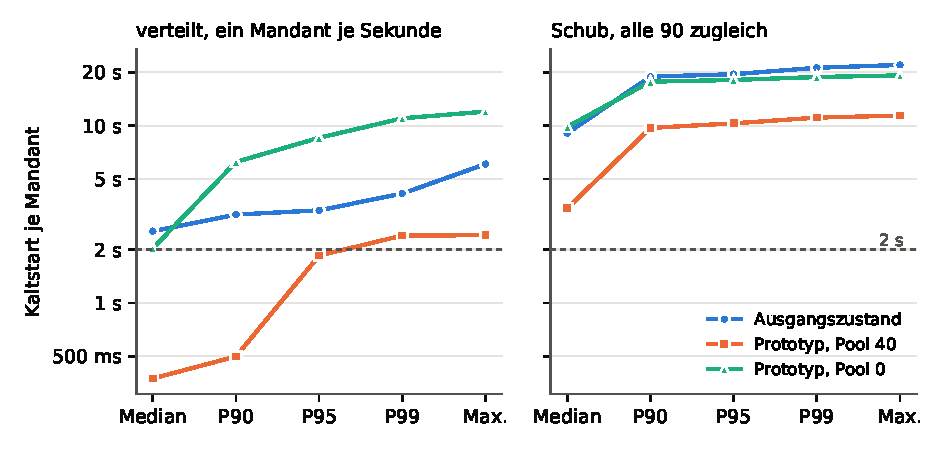
\includegraphics[width=0.8\textwidth]{kaltstart_vergleich.pdf}
  \caption{Kaltstart je Mandant auf hyper-int-otc nach Perzentilen, logarithmische Achse, Werte aus
    \autoref{tab:kaltstart-vergleich}. Die gestrichelte Linie markiert zwei Sekunden.}
  \label{fig:kaltstart-vergleich}
\end{figure}

Je Spalte sind es 90 Mandanten mit je einem Aufruf, beim Ausgangszustand im verteilten Lauf 91, und P99 entspricht
praktisch dem Maximum. Intervalle für P95 und die Anteile unter zwei Sekunden stehen in \autoref{tab:kaltstart-ki}. Sie
setzen unabhängige Werte voraus und erfassen im Schub nur die Unsicherheit durch n = 90, nicht die Streuung zwischen Schüben.

Im verteilten Lauf liegt der Prototyp mit Pool im Median bei 344\,ms gegen 2,54 Sekunden, ein Faktor von gut sieben,
und bedient alle 90 statt 10 von 91 Mandanten innerhalb von zwei Sekunden. Am 15.\ Oktober, vor der Trennung in
Transport und Sandbox, liegen Median und 95.\ Perzentil bei 375\,ms und 1,85 Sekunden, direkt nach der Trennung bei
552 und 890\,ms. Die Bewertungsregel stand vorab fest. Der Entwurf wurde bis zum 26.\ Oktober abgestimmt. Drei Änderungen am
Erstkontakt senkten sie auf 344 und 525\,ms: Der Transport verbindet sich bei der
Zuweisung sofort mit NATS, die Control Plane legt den Consumer parallel zur Zuweisung an, und Transport und Sandbox
führen ihren ersten \ac{TLS}-Handshake schon beim Start aus. Er kostet unter gVisor rund 75\,ms. Im Schub bekommen
genau vierzig Mandanten einen Worker innerhalb von zwei Sekunden, die Zielgröße des Pools. Die übrigen fünfzig
warten bis zu acht Sekunden auf neue Pods. Dort müssen beide Modelle Pods starten. Der Prototyp bleibt mit
höchstens 8,0 gegen 22,0 Sekunden schneller und ohne Fehler.  Die Control Plane legt 48 Pods in 0,18 Sekunden an, der
Start der Container streut auf den Knoten über 1,1 bis 7,3 Sekunden. Alle 17 Fehler des Ausgangszustands,
16 aus der Tabelle und einer aus dem Aufwärmlauf mit neun Mandanten, sind
502 mit \enquote{no route to host} zum Queue-Proxy eines Runner-Pods. Das deutet darauf hin, dass Knative frische Pods
anspricht, bevor ihr Netz erreichbar ist. Belegt ist das nicht. Die Wiederholung vom 28.\ Oktober mit dem Egress-Proxy
liegt im verteilten Lauf bei 416\,ms im Median und 517\,ms im 95.\ Perzentil, 89 von 90 Mandanten bleiben unter zwei
Sekunden (Maximum 2,41 Sekunden, nicht zerlegt). Im Schub sind es 3,93 und 7,52 Sekunden, ohne Fehler. Der Proxy macht den
Kaltstart nicht messbar teurer.

Die Läufe mit Pool null ordnen den Vorsprung ein. Ohne vorgehaltene Pods startet der Prototyp etwa so schnell wie der
Ausgangszustand, im verteilten Lauf 2,03 gegen 2,54 Sekunden im Median, im Schub 9,85 gegen 9,06. Der Vorsprung
stammt damit aus dem Pool und nicht aus einem schnelleren Startmechanismus. Ohne Pool bleibt die Zuverlässigkeit:
null von 188 Aufrufen scheitern gegen 17 von 190 beim Ausgangszustand, jeweils einschließlich eines Aufwärmlaufs mit acht
beziehungsweise neun Mandanten. Dass der Tail mit 8,5 Sekunden im 95.\
Perzentil länger ist als bei Knative, liegt nach den Logs der Control Plane daran, dass ein wartender Mandant den
nächsten bereiten Pod nimmt, nicht den für ihn angelegten, und im ungünstigen Fall bis zu zwölf Sekunden verliert. Die
Vergabe an den am längsten wartenden Mandanten ist in \autoref{sec:betriebsplanung} als offene Maßnahme vermerkt.
 

Für das Agentenprofil gibt es keinen Ausgangswert. Als Richtwert wurden am 21.\ Oktober 2026 dreißig Mandanten im
Sekundentakt erstmals über den Endpunkt der Agentenausführungen aufgerufen, mit einem Snippet, das nur rechnet:
Median 623\,ms, 95.\ Perzentil 816\,ms, alle unter zwei Sekunden. Zweihundert aufeinanderfolgende warme Aufrufe
liegen im Median bei 148\,ms und im 95.\ Perzentil bei 181\,ms.

\subsection{Overhead und warme Latenz (S2)}
\label{sec:warm}

\autoref{tab:overhead} stellt die Läufe mit dem Lastprofil gegenüber. Weil das Profil die
Mandanten überwiegend aktiv hält, nähert der Overhead die warme Latenz an und enthält einen
kleinen Anteil Erstkontakte.

\begin{table}[H]
  \caption{Overhead im Lastprofil auf hyper-int-otc in Millisekunden, k6, je Lauf rund 33 Minuten}
  \label{tab:overhead}
  \footnotesize
  \begin{tabularx}{\textwidth}{@{}l >{\RaggedRight\arraybackslash}X r r r r r r r@{}}
    \hline
    Lauf & Modell, Modus & Aufrufe & Fehler & P50 & P90 & P95 & P99 & Max \\
    \hline
    18 & Ausgangszustand, Profil & 56.976 & 408 & 259 & 1.190 & 2.310 & 4.570 & 50.530 \\
    20 & Prototyp, Wide & 68.881 & 1$^{a}$ & 131 & 257 & 306 & 373 & 3.960 \\
    28 & Prototyp, Profil & 57.001 & 0 & 127 & 164 & 180 & 268 & 15.460 \\
        30 & Prototyp, Profil, mit Reconnect & 57.001 & 8$^{b}$ & 127 & 163 & 178 & 276 & 5.580 \\
    26.10. & Prototyp nach der Trennung in Transport und Sandbox, Profil & 57.001 & 0 & 128 & 165 & 183 & 434 & 3.404 \\
        26.10. & Prototyp, Control Plane beendet den Leerlauf, Profil & 57.001 & 14$^{c}$ & 138 & 239 & 293 & 405 & 3.443 \\
    28.10. & Ausgangszustand, Profil, Ingress-Limit angehoben & 56.989 & 6$^{d}$ & 301 & 490 & 746 & 3.410 & 16.500 \\
    28.10. & Prototyp mit Egress-Proxy, Profil & 57.001 & 0 & 155 & 253 & 296 & 399 & 12.260 \\

    \hline
    \multicolumn{9}{@{}p{\textwidth}@{}}{\footnotesize $^{a}$ clientseitig, Status 0. $^{b}$ 7
      clientseitig, 1 Plattform. $^{c}$ alle Status 502 mit \enquote{sandbox unavailable}, Verbindung zur Sandbox auf dem Loopback verweigert, in den Perzentilen der 56.987
      übrigen Aufrufe nicht enthalten. $^{d}$ alle 502 \enquote{no route to host} in der ersten Minute.} \\
  \end{tabularx}
\end{table}

\begin{figure}[H]
  \centering
  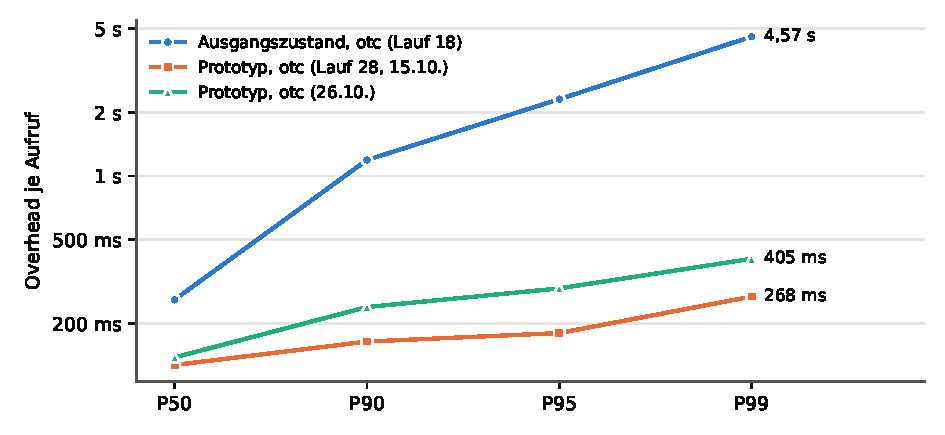
\includegraphics[width=0.75\textwidth]{overhead_lastprofil.pdf}
  \caption{Overhead im Lastprofil nach Perzentilen, Lauf 18 und 28.\ Oktober des Ausgangszustands, 26.\ und 28.\ Oktober des
    Prototyps, logarithmische Achse, Werte aus \autoref{tab:overhead}}
  \label{fig:overhead}
\end{figure}

Auf demselben Cluster und unter demselben Profil liegt der Prototyp am 28.\ Oktober, mit Egress-Proxy, im Median bei
155\,ms gegen 301\,ms des Ausgangszustands, im 95.\ Perzentil bei 296\,ms gegen 746\,ms und im 99.\ bei 399\,ms gegen
3,41 Sekunden. Das ist das 1,9-, 2,5- und 8,5-Fache. Der Ausgangszustand lief diesmal bei angehobenem Ingress-Limit.
Höchstens zwei Pods warteten gegen 54 in Lauf 18, und die sechs Fehler sind 502 in der ersten Minute beim Hochfahren.
Ob der Ingress neu startete, ist ohne Zugriff auf seinen Namespace nicht belegt, die Fehlerzahl spricht dagegen. In Lauf 18
hatte der Neustart des einzigen Ingress-Pods bei 790 von 800\,MiB den größten Teil der 408 Fehler verursacht. Der Prototyp hat in den Läufen 28 und 30 keinen beziehungsweise einen Fehler der Plattform. Die
übrigen Fehler sind clientseitige Abbrüche und 504 des Edge-Proxys, hinter denen das Gateway nachweislich 200
geantwortet hatte. Sie treffen beide Modelle. Der Unterschied im Median liegt zwischen einem Node.js-Prozess hinter einer
Knative-Route und einem Isolate in einem laufenden Worker und trägt nach \autoref{sec:messaufbau} auch die
verschiedenen Begleitdienste. Der Unterschied im Tail entsteht beim Hochfahren von null. Der Wide-Lauf lief noch mit dem
Executor vor den Korrekturen aus \autoref{sec:zuverlaessigkeit} und ist mit Lauf 28 nicht vergleichbar.

Gegenüber dem 26.\ Oktober (128\,ms im Median) kostet der Proxy 27\,ms. Nach der Zerlegung in Tempo (Quantile je Span,
28.\ gegen 26.\ Oktober) brauchen Anmeldung und Abmeldung der Ausführung beim Proxy je rund 11\,ms im Median und
höchstens 17\,ms im 99.\ Perzentil, zusammen 22,5\,ms im kritischen Pfad. Die Abmeldung läuft vor der Antwort, nach ihr
sparte sie 11\,ms. Der Anstieg im 90.\ und 95.\ Perzentil um 90 bis 110\,ms stammt nicht vom Proxy, sondern vom Zugriff
auf S3 im Resolve des Skriptdienstes (P95 von 7,8 auf 118\,ms), den beide Modelle nutzen. Executor und Sandbox sind an
beiden Tagen gleich.

Von den 150 langsamsten Aufrufen im ersten Lauf vom 26.\ Oktober sind 111 Erstkontakte und 26 Aufrufe an Mandanten, deren
Worker sich wegen Leerlaufs gerade beendet hatte. Seit die Control Plane den Leerlauf selbst beendet, sinkt die Zahl der
Aufrufe mit mindestens einer Sekunde Overhead von 37 auf 25.

Wo die Zeit innerhalb des Prototyps entsteht, zeigt die Zerlegung von je vierzig Traces vom 6.\ Oktober in
\autoref{tab:anfragepfad} im Anhang. Der Worker trägt bei zehn wie bei vierzig Aufrufern rund 17\,ms. Die
Verdopplung der Gesamtzeit entsteht im Warten darauf, dass der Skriptdienst das Resolve aufnimmt. Das liegt außerhalb des
Ausführungsmodells. Innerhalb des Workers liegt die Ausführung nach dem Histogramm des Executors im Median
bei 19,3\,ms, im 90.\ Perzentil bei 39,2\,ms und im 99.\ bei 88,4\,ms. Die Erzeugung des Isolates aus dem Snapshot
braucht im Median 15,6\,ms.  Die Erzeugung macht
damit rund vier Fünftel der Ausführung aus und ist der Preis der Isolate-Grenze aus \autoref{sec:ebenen}. Das in
\autoref{sec:betriebsplanung} genannte vorab erzeugte Isolate würde ihn vom Anfragepfad nehmen, ohne M2
aufzugeben.

\subsection{Durchsatz und Ressourcenbedarf (S4, S3)}
\label{sec:durchsatz}

Für S4 stieg die Ankunftsrate in Stufen von je 60 Sekunden um 100 Aufrufe je Sekunde, nach einem Warm-up mit 50
Aufrufen je Sekunde und über 100 Mandanten mit je einem Skript. Als Wert gilt die höchste Stufe mit einer
Fehlerrate unter einem Prozent und einem 95.\ Perzentil unter zwei Sekunden. k6 lief als Job im Namespace des
jeweiligen Modells. Beide Modelle liefen ohne Signatur- und \ac{IdP}-Prüfung über je eine Kopie des Einstiegsdienstes, die
nur für diesen Test bestand. Der Ausgangszustand lief mit vier festen Replikas des Skriptdienstes, weil sich der
Autoscaler nicht anlegen ließ, was Knative leicht begünstigt.

\begin{table}[H]
  \caption{Durchsatz (S4) auf hyper-int-otc, höchste Stufe mit Fehlerrate unter einem Prozent und
    P95 unter zwei Sekunden}
  \label{tab:s4}
  \small
  \begin{tabularx}{\textwidth}{@{}>{\RaggedRight\arraybackslash}X r >{\RaggedRight\arraybackslash}X@{}}
    \hline
    Konfiguration & Stufe & Nächste Stufe \\
    \hline
    Ausgangszustand & 100/s & 200/s: 1,28\,\% Fehler (HTTP 500) \\
    Prototyp, Gateway wie ausgerollt (200\,m, 128\,MiB) & 200 bis 300/s & 400/s: Gateway beendet (\texttt{OOMKilled}),
      bis 50\,\% Fehler \\
    Prototyp, Gateway 1 Kern und 512\,MiB, drei Replikas für den Resolve & 500/s & 600/s: P95 4,4 bis
      10\,s \\
    \hline
  \end{tabularx}
\end{table}

Der Prototyp hält damit 500 Aufrufe je Sekunde gegen 100 im Ausgangszustand. Seine Grenze liegt nicht in der
Ausführung, die Worker verbrauchen zusammen 10 bis 15 Kerne, sondern in der Architektur der bestehenden App. Mit dem
ausgerollten Gateway und einer Replika für den Resolve liegt sie bei 200 bis 300 Aufrufen, mit größerem Gateway und
drei Replikas, wie der Skriptdienst sie im Betrieb erhält, bei 500. Darüber wartet der Resolve im Stream auf einen
freien Slot (3,1 Sekunden bei 600 Aufrufen gegen 42 bis 85\,ms Bearbeitung). Die Datenbank des Skriptdienstes
liegt bei 81 bis 89 Prozent \ac{CPU} und 92 Prozent der Verbindungen. Im Ausgangszustand begrenzt dagegen die
Ausführung: Ab 400 Aufrufen je Sekunde starten zusätzliche Runner, bis über 300 Pods. Die Stufen sind 100 Aufrufe
breit, der Wert ist eine untere Schranke, und je Konfiguration gibt es ein bis drei Läufe.

S3 wird je Pod erhoben, weil der Ausgangszustand je Ausführung ohnehin einen ganzen Pod belegt und ein Worker-Pod
mehrere Ausführungen zugleich trägt. Verglichen wird die Kaltstartmessung auf hyper-int-otc
(\autoref{tab:ressourcen-vergleich} im Anhang), in der beide Modelle unter gVisor laufen und cAdvisor die Pod-Ebene
erfasst. Am 26.\ Oktober wurde der Speicher nach der Trennung in Transport und Sandbox wiederholt
(\autoref{tab:ressourcen-trennung}). Ein Runner-Pod des Ausgangszustands belegt mit 90\,MiB im Median rund das
Eineinhalbfache eines Worker-Pods mit 59\,MiB, der vor der Trennung bei 46\,MiB lag. Der zweite Prozess kostet also
rund 13\,MiB. Die \ac{CPU} unterscheidet sich kaum, beide Pods sind die meiste Zeit untätig. Die Steuerungsschicht
fällt stärker auseinander: Knative Serving mit Kourier hält rund 1,4\,GiB in sieben Pods, Control Plane und Gateway
des Prototyps 113 bis 167\,MiB, rund ein Neuntel. Der Pool kostet nach der Messung vom 15.\ Oktober dauerhaft rund 1,9\,GiB und 0,75
Kerne, bei 59 statt 46\,MiB je Pod hochgerechnet rund 2,3\,GiB, etwa so viel wie Knative Serving selbst, und kauft damit die
Kaltstarts. Ruhende Mandanten kosten im Ausgangszustand nichts, im Prototyp den Pool. Ohne Pool hat der Prototyp mit 8,2
gegen 13,7\,GiB die niedrigste Spitze. cAdvisor wird nur etwa alle 70 Sekunden
abgefragt, und NATS mit 0,21 bis 0,25 Kernen ist dem Prototyp nicht zugerechnet. Pod-Zahl, Gesamtspeicher und
\ac{CPU} je Pod sind für den 26.\ Oktober nicht belastbar, weil der Wechsel auf Pool null das Fenster mit Pool 40
verkürzte.

\subsection{Zuverlässigkeit der Zustellung}
\label{sec:zuverlaessigkeit}

Bis zum 26.\ Oktober stellten die Consumer jede Nachricht höchstens einmal zu, weil eine Skriptausführung nicht
idempotent ist. Die Läufe zeigen die Kehrseite: Eine Nachricht, die ein Worker entgegennimmt und nicht
behandelt, ist verloren, und der Aufrufer wartet bis zum Timeout. \autoref{tab:zustellung} im Anhang führt die sechs
Fälle auf, in denen Aufrufe verloren gehen oder erst nach dem Timeout laufen. Jeder wurde über die Trace-Kennung bis
zur Ursache verfolgt.  Drei der sechs Fälle haben dieselbe Form: Ein Pull, in den der Server noch zustellen kann, wird vom
Worker aufgegeben, durch Prozessende, einen verworfenen Pull oder einen Pull ohne Leader. Unter einer einzigen Zustellung
ruhte die Korrektheit damit auf der Disziplin des Workers, eine zugestellte Nachricht nie aufzugeben. Die
Festlegung, je Nachricht genau einen Pull zu ziehen und sich nur zwischen zwei Pulls zu beenden, ist das Ergebnis dieser
Läufe. Seit dem 27.\ Oktober käme sie nach fünf Sekunden zurück. Gemessen ist das nur beim Knotenentzug (\autoref{sec:pruefung-m5}). Zwei Fälle liegen außerhalb des Entwurfs:
das Consumer-Limit des Kontos und ausbleibende Antworten auf langlebigen Verbindungen. Die Ursache der ausbleibenden
Antworten ist offen. Für sie bleibt der Reconnect ein Workaround. Der
verbleibende Fall zeigt eine zweite Lücke: Skripte laufen 111 bis 173 Sekunden nach dem Aufruf, wenn der Aufrufer
längst aufgegeben hat. Seit dem 27.\ Oktober verwirft der Worker sie ungelaufen (\autoref{sec:zuteilung}), ungemessen.


\subsection{Isolation und Zustandsfreiheit (M1 bis M4)}
\label{sec:pruefung-isolation}

M1 und M3 werden durch Architektur- und Konfigurationsvergleich geprüft, M1 über die Ebenen der Trennung aus
\autoref{sec:ebenen} und den Prüffall T10, M3 über den Vergleich der Pod-Spezifikation des Workers mit der des Ausgangszustands. M2 und M4
werden über die Prüffälle T1 bis T9 aus \autoref{tab:prueffaelle} geprüft, als Skripte gegen den Ausgangszustand und
den Prototyp. Ein Prüffall gilt als bestanden, wenn der Zugriff scheitert oder der Zustand die nächste Ausführung
nicht erreicht. Beide Varianten wurden am 19.\ Oktober auf hyper-int-otc mit demselben Mandanten geprüft, der für den
Ausgangszustand über die App-\acs{URL} auf den Knative-Stack umgestellt und danach zurückgestellt wurde. Jeder
Prüffall ist ein eigenes Skript, das über die öffentliche Adresse des Mandanten aufgerufen wird, wie ein echter
Webhook. T1 bis T5 rufen dasselbe Skript dreimal hintereinander auf. Jede Ausführung meldet, was sie von der vorigen
vorfindet, und legt eigenen Zustand ab. T6 fordert Speicher an, bis die Laufzeit abbricht, und ruft danach fünfmal ein
zweites Skript desselben Mandanten auf. T7 bis T9 laufen einmal und protokollieren je Zugriffsweg, ob er gelingt. T9
überschreibt vorher jede Kopie der Mandantenidentität. Inhalte von Dateien oder Umgebungsvariablen werden nicht
ausgelesen.

\begin{table}[tbp]
  \caption{Prüffälle T1 bis T9 gegen Ausgangszustand und Prototyp, hyper-int-otc, 19.\ Oktober}
  \label{tab:prueffaelle-ergebnis}
  \footnotesize
  \begin{tabularx}{\textwidth}{@{}l l l >{\RaggedRight\arraybackslash}X@{}}
    \hline
    Nr. & Ausgangszustand & Prototyp & Beobachtung \\
    \hline
    T1 & nicht bestanden & bestanden & Knative: Ein Intervall aus Ausführung $n$ schreibt in ein
         Objekt, das Ausführung $n+1$ angelegt hat. Prototyp: Das Objekt bleibt unberührt. \\
    T2 & nicht bestanden & bestanden & Knative: Globale Variablen aus $n$ sind in $n+1$ lesbar,
         obwohl das Modul neu ausgewertet wird. Prototyp: nicht vorhanden. \\
    T3 & nicht bestanden & bestanden & Knative: Änderungen an \texttt{Array.prototype},
         \texttt{Object.prototype}, \texttt{JSON.parse}, am Modul \texttt{crypto} und an
         \texttt{require.cache} wirken fort, nur \texttt{path} kommt frisch. Prototyp: keine wirkt
         fort, \texttt{require.cache} existiert nicht. \\
    T4 & bestanden & bestanden & Beide: Die Datei aus $n$ fehlt in $n+1$. Knative setzt das
         temporäre Verzeichnis zurück, der Prototyp beginnt jede Ausführung mit leerem
         Dateisystem im Speicher. \\
    T5 & nicht bestanden & bestanden & Knative: Die in $n$ geöffnete \acs{TLS}-Verbindung ist in
         $n+1$ offen und beantwortet eine neue Anfrage mit 200. Prototyp: nicht auffindbar. \\
    T6 & nicht bestanden & bestanden & Knative: Der Prozess stürzt nach 10,3\,s ab, die nächste
         Ausführung scheitert mit 502, erst danach antwortet ein neu gestarteter Prozess.
         Prototyp: Abbruch nach 0,36\,s mit eigenem Fehler, die fünf folgenden Ausführungen
         liefern 200. \\
    T7 & nicht bestanden & bestanden & Knative: \texttt{fetch} ins Internet liefert 200,
         \acs{TCP} zur Kubernetes-\acs{API} und zum Port des eigenen Runners wird aufgebaut.
         Prototyp, vor dem Egress-Proxy: Jedes Ziel außer dem eigenen Mandanten wird abgewiesen, und
         \texttt{Deno.core.ops} ist nicht erreichbar. \\
    T8 & bestanden & bestanden & Beide: \texttt{/etc}, \texttt{/proc} und das Token des
         Service-Accounts sind nicht lesbar, im Ausgangszustand durch das Permission Model von
                  Node.js. Knative reicht 23 Umgebungsvariablen an das Skript durch, der Prototyp keine. \\
        T9 & nicht bestanden & bestanden & Beide: Alle Überschreibungen gelingen im Skript. Knative:
         Der Host eines anderen Mandanten ist vorher wie nachher erreichbar, es gibt keine
         Prüfung, an der eine Identität hinge. Prototyp: eigener Host 200, fremder Mandant vorher
         wie nachher abgewiesen, gefälschte Header ändern nichts. \\
    \hline
  \end{tabularx}
\end{table}

\autoref{tab:prueffaelle-ergebnis} zeigt, dass der Prototyp alle neun Prüffälle besteht und der
Ausgangszustand sieben nicht. Die Fehlschläge im Ausgangszustand gehen bis auf T7 und T9 auf dieselbe
Ursache zurück, den gemeinsamen Node.js-Prozess (\autoref{sec:angreifermodell}), auch T6, denn ein erschöpfter Heap
beendet den gemeinsamen Prozess. T4 und T8 besteht der Ausgangszustand, weil er das temporäre Verzeichnis zurücksetzt und
das Permission Model von Node.js das Dateisystem sperrt. Die 23 durchgereichten Umgebungsvariablen zeigen, dass das
Skript dort Konfiguration des Runners sieht.

Dieselben neun Prüffälle liefen am 21.\ Oktober 2026 im Agentenprofil des Prototyps auf einem zweiten
Testmandanten, als Snippets über den Endpunkt der Agentenausführungen, übertragen auf die Mittel des Profils
(Prototypen und Globals, dynamische Importe, \texttt{fetch}), weil es weder \texttt{require} noch \texttt{process}
noch eine Konsole bereitstellt. Der Ausgangszustand hat dafür kein Gegenstück. T1 bis T3 liefen zusätzlich mit zwei
gleichzeitigen Ausführungen. Der Prototyp besteht alle neun Fälle. Zustand erreicht keine andere Ausführung, auch
keine gleichzeitige (T1 bis T3, ohne Aussage zu Seitenkanälen zwischen den bis zu vier Isolates eines Prozesses,
\autoref{sec:betriebsplanung}). Module, Dateisystem und Betriebssystem lassen sich nicht laden (T4, T8).
\texttt{fetch} scheitert zu jedem Ziel, auch vor und nach dem Überschreiben aller erreichbaren Kopien der Identität
(T5, T7, T9). Die Speicherbombe endet nach 0,3 Sekunden mit dem Fehler \texttt{scriptExecutionOutOfMemory}, die
fünf folgenden Ausführungen liefern 200 (T6).

T7 und T9 wurden am 28.\ Oktober gegen den Egress-Proxy mit beiden Profilen in enforce wiederholt, mit der Testregel
example.org:443. Jeder Lauf erreicht zusätzlich das eigene System. Im Webhook-Profil gehen der eigene Mandant und die
Testregel durch. Abgewiesen werden example.com, \texttt{http://1.1.1.1}, TCP zu 1.1.1.1:53, die Testregel auf Port 80,
\texttt{kubernetes.default.svc}, die Metadaten-Adresse, der Loopback und der Tunnel zu \texttt{nats:4222}.
\texttt{Deno.core.ops} ist nicht erreichbar, T9 besteht wie zuvor. Im Agentenprofil mit einer Regel des Aufrufers
(example.net, GET) gehen der eigene Mandant, diese Regel mit GET und die Testregel durch. Abgewiesen werden dieselbe Regel
mit POST, example.com, ein fremder Mandant, 1.1.1.1 und die internen Ziele, und das Anfrageprotokoll der Antwort führt
alle Versuche, die abgewiesenen mit 403. Beide Profile bestehen, die Politik wirkt also, nicht nur der Durchsetzungspunkt.
Geprüft ist eine feste Testregel, kein Regelwerk eines Mandanten.

Ergänzend wurden die 51 Eigenschaften von SandboxEval \autocite[S.~1--2]{rabin_sandboxeval_2025} für JavaScript
angepasst und auf dem Ausgangszustand und beiden Profilen des
Prototyps ausgeführt. Das Original ist auf Python und Linux zugeschnitten.
\autoref{tab:sandboxeval} im Anhang zählt die Fälle, die ohne Fehler antworteten. Im
Ausgangszustand geben 12 davon Information über den echten Host preis, und fünf erreichen externe Ziele. Im Webhook-Profil des Prototyps antworten
29 Fälle mit leeren oder nachgebildeten Werten, und keiner erreicht ein externes Ziel. Im Agentenprofil antworten
zwei, die Zeitzone und eine Rechenschleife.

Der Konfigurationsvergleich für M3 (\autoref{tab:m3} im Anhang) stellt die Felder gegenüber, die die dem Gastcode
zugängliche Kernel-Oberfläche bestimmen. Sie stammen aus laufenden Pods auf
hyper-int-otc vom 20.\ Oktober 2026, aus dem Container, der den Gastcode ausführt, und stimmen mit der Pod-Spezifikation im
Quellcode überein. Das Plattform-Team stellt gVisor nur auf \ac{OTC} bereit. Die
Control Plane setzt die Runtime-Klasse deshalb nur, wenn der Name der Infrastruktur \texttt{otc} enthält, und startet dort
nicht, wenn ein Worker-Pod im Trockenlauf ohne die Klasse ankäme. Der Vergleich gilt für hyper-int-otc.
In keiner Zeile ist der Prototyp lockerer als der Ausgangszustand: Sechs Felder sind
gleich, zwei sind zusätzlich gesetzt. Sie beschränken, was der Prozess im Container verändern kann, nicht die
Systemaufrufe, die gVisor annimmt. M3 ist damit auf Clustern mit gVisor erfüllt. Die Aussage stützt sich auf die
Konfiguration und sagt nichts über Lücken in gVisor selbst. M1 ist im Entwurf mit Auth Callout erfüllt (T10), im gemessenen Plattformstand nicht: Ein Ausbruch aus Engine und Container erreicht ohne den Callout die gemeinsamen
NATS-Zugangsdaten. Der Callout ist auf der Plattform noch nicht eingerichtet
(\autoref{sec:betriebsplanung}). Am Cluster ist am 28.\ Oktober die Pod-Spezifikation geprüft: Die Container teilen
keinen Prozess-Namespace, die Sandbox hat keine Volumes, und Identitätssecret und NATS-Zugangsdaten sind nur im
Transport eingehängt, ohne Token des Service-Accounts. Das Netz teilen beide Container. Dass der Transport fremde
Kommandos abweist und NATS ohne Zugangsdaten nichts zulässt, ist nur lokal geprüft.

Der Prüffall T10 prüft M1 und lief am 28.\ Oktober 2026 lokal mit Auth Callout, weil auf hyper-int-otc keiner läuft. Der Code
hat die Netz- und Prozesssicht des Sandbox-Containers, also die Lage nach einem angenommenen Ausbruch aus V8. Im
Sandbox-Prozess liegen keine Zugangsdaten. Eine Verbindung zu NATS ohne Zugangsdaten, mit der Worker-Kennung, mit einem geratenen Passwort und mit einem gefälschten Token
endet jeweils in einer \enquote{Authorization Violation}, der Callout nennt im Log \enquote{no assignment token}
beziehungsweise \enquote{invalid assignment token}. Ein Zuweisungsbefehl an den eigenen Transport über Loopback und über
die Pod-\ac{IP} erhält \ac{HTTP} 403, derselbe Befehl an den Transport eines anderen Workers scheitert an der
Netzwerkrichtlinie. T10 ist bestanden. Die Rechte einer gültigen Verbindung auf andere Mandanten sind nicht geprobt, die Rechteliste des
Callouts belegt sie (\autoref{lst:callout-rechte}).

\subsection{Verfügbarkeit beim Knotenentzug (M5)}
\label{sec:pruefung-m5}

Ein rollierendes Knotenupdate evakuiert die Pods eines Knotens über \texttt{kubectl drain}
\autocite{the_kubernetes_authors_safely_2026}. Auf dem geteilten Integrationscluster steht das nicht zur Verfügung.
Deshalb löscht der Ersatz unter Last alle Worker-Pods eines Knotens im Namespace, sodass jeder wie bei einer Eviction
SIGTERM und seine Grace Period erhält und die Control Plane die Löschung über den Informer sieht. Nicht abgebildet
ist, dass ein Drain auch Control Plane, Gateway und NATS-Server desselben Knotens evakuiert. Sie sind Deployments
mit Repliken und nicht Gegenstand von M5. Erhoben werden je Mandant die Zeit von der Löschung bis zur ersten danach
begonnenen erfolgreichen Ausführung, die Zahl der verlorenen Aufträge und ob eine Ausführung, die die Löschung
überspannt, zu Ende läuft. Der Ausgangszustand wird mit demselben Ersatz gemessen, indem der Runner-Pod des Mandanten
gelöscht wird. Seine Zeit ohne Ausführungsfähigkeit ist der Zielwert aus \autoref{sec:kriterienkatalog}. Acht Mandanten setzten Schlag auf Schlag kurze Aufrufe ab, die Löschung folgte 90 Sekunden nach Laufbeginn, ein Lauf
dauerte 240 Sekunden. Jeder Mandant hielt zusätzlich lange Aufrufe von 25 Sekunden Haltezeit vor, von denen einer die
Löschung überspannte.  Der Pool hielt vierzig freie Pods.

Die erste Reihe vom 19.\ und 20.\ Oktober (\autoref{tab:m5} im Anhang) lief vor der Trennung in Transport und Sandbox mit
kurzen Aufrufen von rund 1,2 Sekunden. Die Lücke der getroffenen Mandanten liegt zwischen 0,61 und 1,37 Sekunden, im Bereich
der nicht getroffenen, es gibt keinen Fehler und keinen verlorenen Auftrag, und alle 32 langen Aufrufe über die Löschung
enden mit 200 nach rund 25 Sekunden. Der Ausgangszustand, ein Lauf mit einem Mandanten, hat 1,9 Sekunden. Die Reihe
löst nur auf 1,2 Sekunden auf. Die zweite Reihe vom 28.\ Oktober ersetzt die kurzen Aufrufe durch einen Prober: Je Mandant
ein Skript ohne Haltezeit, alle 100\,ms über vier Keepalive-Verbindungen. Gemessen wird der längste Abstand zweier
erfolgreicher Antworten nach der Löschung. In vier Läufen des Prototyps mit 14 getroffenen Mandanten-Läufen beträgt er
0,21 bis 0,42 Sekunden und liegt damit nahe an der Netzlaufzeit von rund 0,2 Sekunden. In vier Läufen des Ausgangszustands
mit zehn Mandanten-Läufen sind es 2,10 bis 2,69 Sekunden: Die gelöschten Runner bedienen noch kurz, danach zahlen neue
Aufrufe den Kaltstart der ersetzten Runner. Kein Modell verliert eine Ausführung. Der relative Zielwert aus
\autoref{sec:kriterienkatalog} ist erreicht. Ein echtes Drain, bei dem viele Pods zugleich weichen, kann länger dauern und
ist auf dem Integrationscluster nicht messbar.

Die Reihe deckte einen Fehler im Executor auf. Bis zum Fix am 28.\ Oktober um 16:04 \ac{UTC} wurden Ausführungen, die bei
der Löschung liefen, nach 3,5 bis 4 Sekunden neu zugestellt und von vorn ausgeführt, sechs lange Aufrufe endeten nach 33
bis 36 statt 25 Sekunden. Die Verbindung, die den Transport mit der Sandbox hält, steckte in einem \texttt{select!}-Zweig,
den SIGTERM verwarf, sodass die Sandbox sich nach den Logs 3\,ms nach dem Signal beendete. Der Fehler kam mit der Trennung
in Transport und Sandbox und ist kein Mangel des Entwurfs. Nach dem Fix enden 8 von 8 langen Aufrufen über die Löschung
nach 25,2 Sekunden mit 200, und die Sandbox schließt erst rund 20 Sekunden später nach dem Drain. Beim Knotenentzug geht
damit keine Ausführung verloren und keine läuft doppelt. Für den Absturz eines Workers gilt das nicht
(\autoref{sec:zuteilung}).

\subsection{Kompatibilität des Bestands (S6, S7)}
\label{sec:pruefung-kompatibilitaet}

S6 wird aus der Bestandsanalyse in \autoref{sec:bestandsanalyse} und den Prüfungen der
Kompatibilitätsschicht abgeleitet, nicht durch Ausführen des Bestands gemessen. \autoref{tab:s6} im Anhang leitet die Zahl her. Von den 1.718
Mandanten brauchen 713 eine Schnittstelle, die eine sprachbasierte Laufzeit ohne vermitteltes
Binding nicht bietet, und 648 davon scheitern allein an einem Netzwerk-Binding. Genau diese beiden
Gruppen, \ac{HTTP} und rohe Sockets, bildet die Schicht nach, belegt durch den Differenztest mit
757 Fällen, die Integrationstests und die Machbarkeitsprüfung am schwierigsten Vertreter. Die
übrigen 65 Mandanten brauchen Dateisystem, Betriebssystemmodule oder Prozesse. 16 von ihnen nutzen
nur \texttt{http}, \texttt{https}, \texttt{net} oder \texttt{tls}, die die Schicht nachbildet. Die
Skripte der übrigen 49 wurden gelesen und am 21.\ Oktober 2026 mit einem Probeskript auf dem
Ausgangszustand und dem Prototyp geprüft. 34 schreiben Dateien in das erste Verzeichnis unter \texttt{/tmp}.
Sie scheitern im Probelauf schon im Ausgangszustand, an der Skriptdatei als einzigem Eintrag in \texttt{/tmp}, im Prototyp
am leeren Verzeichnis. Ob der Pfad in Produktion erreicht wird, ist nicht geprüft. Die übrigen 15 Skripte stehen in
\autoref{tab:s6}, ebenso die Wertung der vier gebündelten, nicht unterstützten Skripte (1.713 von 1.718, 99,7 Prozent).
Dass 38 Skripte schon im Ausgangszustand scheitern, ändert dessen fünf Punkte nicht, denn S6 misst den Anteil, der nicht
schlechter läuft als dort. Damit laufen bis zu 1.717 von 1.718 Mandanten, 99,9 Prozent, nicht schlechter als im
Ausgangszustand. Das ist eine Obergrenze unter zwei Annahmen: Die
Schicht hält für die übrigen Pakete, was Differenztest und Treiber-Prüfung für einen Treiber zeigen, und die Ziele der
Skripte sind erreichbar. Das hängt am Egress-Proxy
(\autoref{sec:faehigkeitsmodell}). Im Modus audit lässt er jede öffentliche Adresse und jeden Port durch, in enforce, wie
seit dem 28.\ Oktober auf hyper-int-otc, nur den eigenen Mandanten und die Ziele der Regeln (T7). Ein Skript mit
externen Zielen läuft dann erst mit einer Regel, und wie viele Mandanten das betrifft, ist nicht erhoben. Der Scanner-Lauf
vom 25.\ September 2026 gegen einen frühen Stand der Schicht wird nicht wiederholt, weil er
Bezeichner in nie ausgeführten Zweigen mitzählt und damit nur eine Obergrenze der Blocker liefert.
S7, der Aufwand für den Rest, ist für 64 der 65 Mandanten null, weil keine Anpassung am Skript nötig
ist, und für den letzten nicht gewollt. Der Aufwand für Regeln steht darin nicht, er fällt erst unter enforce an.

Die Machbarkeitsprüfung an \texttt{tedious} aus \autoref{sec:kompatibilitaetsschicht} ist bestanden: Der
unveränderte Treiber verbindet sich über den Socket-Shim mit einer echten Datenbankinstanz, führt eine Abfrage aus und
stellt innerhalb des \ac{TDS}-Datenstroms auf \ac{TLS} um. Beide Ergebnisse sind mehrfach reproduziert und gegen
Negativkontrollen geprüft.

\subsection{Zusammenführung}
\label{sec:nutzwert}

\autoref{tab:nutzwert} sammelt die erhobenen Werte entlang der Soll-Kriterien. Die Fehlerrate
ist kein Kriterium des Katalogs und steht deshalb ohne Gewicht dabei. Die Punkte folgen der
Regel aus \autoref{sec:kriterienkatalog}. Der Ausgangszustand erhält je bewertetem Kriterium drei
Punkte, bei S6 und S7 nach derselben absoluten Regel fünf.

\begin{table}[tbp]
  \caption{Stand der Bewertung entlang der Soll-Kriterien}
  \label{tab:nutzwert}
  \footnotesize
  \begin{tabularx}{\textwidth}{@{}l r >{\RaggedRight\arraybackslash}X >{\RaggedRight\arraybackslash}p{0.24\textwidth} r@{}}
    \hline
    Nr. & Gewicht & Prototyp & Ausgangszustand & Punkte \\
    \hline
    S1 & 0,30 & S1a, Pool 40: verteilt P95 525\,ms, Schub P95 6,90\,s, 40 von 90 unter 2\,s.
      S1b, Pool 0: verteilt P95 8,54\,s, Schub P95 18,1\,s & verteilt P95 3,33\,s,
      Schub P95 19,5\,s, 0 von 90 unter 2\,s, 17\,\% Fehler im Schub & S1a 5, S1b 2,2, S1 4$^{a}$ \\
    S6 & 0,25 & bis zu 99,9\,\% der Mandanten nicht schlechter lauffähig, abgeleitet, Regeln nicht erhoben & -- & 5$^{b}$ \\
        S2 & 0,15 & Overhead P50 / P95 / P99 155 / 296 / 399\,ms
      & 301\,ms / 746\,ms / 3,41\,s & 5$^{c}$ \\
    S3 & 0,10 & 59\,MiB je Worker-Pod unter gVisor (Median), Steuerung 113 bis 167\,MiB, Pool
      1,9\,GiB & 90\,MiB je
      Runner-Pod (Median), Steuerung 1,4\,GiB & 4$^{d}$ \\
    S7 & 0,10 & keine Skriptänderung bei 64 von 65 Mandanten, 1 nicht gewollt, Regelaufwand nicht bewertet & -- & 5$^{f}$ \\
    S4 & 0,10 & wie ausgerollt 200 bis 300 Aufrufe/s, mit größerem Gateway 500 & 100 Aufrufe/s & 5$^{e}$ \\
        Nutzwert & 1,00 & 4,6 & 3,7 & \\
                -- & -- & Fehlerrate 0 bis 14 von rund 57.000, die 14 mit unerreichbarer Sandbox & 6 bis 408 von rund 57.000, in Lauf 18 (0,71\,\%) der
      größte Teil ein Ingress-Neustart & \\
    \hline
    \multicolumn{5}{@{}p{\textwidth}@{}}{\footnotesize $^{a}$ S1a: P95 verteilt Faktor 6,3, Schub 2,8, beide fünf Punkte.
      S1b, Stand vom 15.\ Oktober: Faktor 0,4 (1,2 Punkte) und 1,1 (3,2 Punkte), im Mittel 2,2. S1 je zur Hälfte, 3,6 gerundet 4. $^{b}$ Anteil über 80\,\%. Abgeleitet, nicht
      ausgeführt, ohne den Bedarf an Regeln für enforce. $^{c}$ Faktor 1,9 im Median (4,8 Punkte, gerundet 5), 2,5 im 95.\ und 8,5 im 99.\ Perzentil, Läufe vom 28.\ Oktober, einschließlich der verschiedenen Begleitdienste. $^{d}$ Faktor
      1,5 je Pod, 4,0 Punkte. Der Pool von 1,9\,GiB ist nicht je Pod gerechnet. $^{e}$ Faktor 5,0,
      wie ausgerollt 2 bis 3. $^{f}$ 98,5\,\% der 65 Mandanten ohne Skriptänderung.} \\
  \end{tabularx}
\end{table}

Auf vier der sechs Kriterien erreicht der Prototyp die Höchstpunktzahl, bei S1 und S3 vier Punkte. Die Rangfolge hängt nicht von den Gewichten ab, denn der Prototyp ist bei S6 und S7 gleichauf und bei den
übrigen besser. Nur der Vorsprung von 0,9 ändert sich. Er hängt an S6, das unter enforce von den Regeln abhängt: Bei zwei
Punkten, also höchstens 40\,\% der Mandanten, läge der Prototyp mit 3,85 knapp vor 3,7, bei einem mit 3,6 dahinter. Der
Nutzwert ist das Ergebnis einer Zuordnung, deren Vorbehalte in \autoref{sec:messaufbau} stehen.
